\subsection{Data Generating Process}
A stochastic progress $x_t$ is given by the DGP
\begin{equation}
  \begin{split}
    x_t &= f(t) + \phi x_{t-1}+\varepsilon_t,\\
    \text{with }f(t) &= \mu \neq 0,\ \ \ \ \ |\phi|<1\ \text{and}\ \varepsilon_t\sim iid(0,\sigma^2_\varepsilon)
    \label{eq:xt}
  \end{split}
\end{equation}
$x_t$ is the realization of an ergodic stochastic process if it is stationary and for any point in time $t$ satisfies
\begin{equation}
  \displaystyle{\lim_{T\to\infty}}\left(T^{-1}\sum_{s=1}^TCov(x_t,x_{t+s})\right)=0
\end{equation}
That is, on average the memory of the process is bounded. Thus, covariances goes towards $0$ for two different point in time so that two parts of the same stochastic process can be independent from each other.
\\ \\
By iterative substitution we see that equation \ref{eq:xt} can be rewritten as
\begin{equation}
  \begin{split}
    x_t &= \mu + \phi x_{t-1} +\varepsilon_t \\
        &= \mu + \phi (\mu + \phi x_{t-2}+\varepsilon_{t-1}) +\varepsilon_t\\
        &= \mu (1+\phi) + \phi^2 x_{t-2}+ \phi\varepsilon_{t-1} +\varepsilon_t\\
        &= \mu (1+\phi) + \phi^2 (\mu + \phi x_{t-3}+\varepsilon_{t-2})+ \phi\varepsilon_{t-1}+\varepsilon_t\\
        &= \mu (1+\phi+\phi^2) + \phi^3(x_{t-3})+ \phi^2\varepsilon_{t-2} + \phi\varepsilon_{t-1} +\varepsilon_t\\
        &\vdots \\
        &= \phi^T x_{t-T} + \sum_{s=1}^T\left( \mu\phi^{s-1} + \phi^{s-1}\varepsilon_{t-s+1} \right)\\
        &\text{rewriting the sum of the geometric series:}\\
        &= \phi^T x_{t-T} + \mu\left(\frac{1-\phi^T}{1-\phi}\right) + \sum_{s=1}^T \phi^{s-1}\varepsilon_{t-s+1},\\
        &\ \text{where $T$ is the number of periods $s$ prior to $t$.}
        \label{eq:iterative}
  \end{split}
\end{equation}
If the process was a unit root the constant terms with $\mu$ would accumulate and produce a deterministic trend, but as $|\phi|<1$ then $\phi^T\xrightarrow[T\rightarrow\infty]{}0$ such that for a high number of periods $T$ equation \ref{eq:iterative} converges to
\begin{equation}
  \begin{split}
    x_t \xrightarrow[T\rightarrow\infty]{} \frac{\mu}{1-\phi} + \sum_{s=1}^T \phi^{s-1}\varepsilon_{t-s+1}
  \end{split}
\end{equation}
And as $\varepsilon_t$ is a stochastic term the expexted realization of $_t$ will be
\begin{equation}
  \begin{split}
    E(x_t) = \frac{\mu}{1-\phi}
    \label{eq:mean}
  \end{split}
\end{equation}
As the expected mean is a constant then $\{x_t\}_{t=1}^T$ is an integrable $iid$ stochastic process and for $\mu<0$ the Law of large numbers implies that the mean converge in probability
\begin{equation}
  \bar{x}_T\xrightarrow{p}\frac{\mu}{1-\phi}
\end{equation}
Furthermore, we assume $T\rightarrow\infty$ then $x_t$ can be rewritten to a sequence of random variables $\{\tilde{x}_T\}_{T=1}^\infty$ that are drawn   from a population with a probability distribution with finite mean $\frac{\mu}{1-\phi}$ and finite variance $\sigma_\varepsilon^2$. The Central Limit Theorem then implies convergence to the normal distribution
\begin{equation}
  \sqrt{T}\left(\bar{x}-\frac{\mu}{1-\phi}\right) \xrightarrow{d}N(0,\sigma_\varepsilon^2)
\end{equation}
The derivations above shows that the memory of $x_t$ is bounded as the stationarity condition $|\phi|<1$ is fullfilled, thus the memory of the initial value $x_{t-T}$ and chock $\varepsilon_{t-T+1}$ decreases to zero the further away in time $t$ is from the initial period $t-T$.

Furthermore, the deterministic term given by the constant $\mu\neq0$ does not give rise to a linear trend, as $|\phi|<1$.

In conclusion, $x_t$ in equation \ref{eq:xt} describes an ergodic stochastic process.

% This is even more clear when applying the difference operator with the order of integration $I(1)$ however would be an ergodic stochastic process as the deterministic parts would cancel each other out.
% \begin{equation}
%   \begin{split}
%     \Delta x_t  &= x_{t} - x_{t-1}\\
%                 &= [\mu + \phi x_{t-1} +\varepsilon_t] - [\mu + \phi x_{t-2} +\varepsilon_{t-1}]\\
%                 &= [\mu + \phi (\mu + \phi x_{t-2}+\varepsilon_{t-1}) +\varepsilon_t] - [\mu + \phi x_{t-2} +\varepsilon_{t-1}]\\
%                 &= \phi \mu + (\phi^2-\phi) x_{t-2} + (\phi-1) \varepsilon_{t-1} +\varepsilon_t\\
%                 &= \phi \mu + (\phi^2-\phi)(\mu + \phi x_{t-3}+ \varepsilon_{t-2}) + (\phi-1) \varepsilon_{t-1} +\varepsilon_t\\
%                 &= \phi^2 \mu + (\phi^3-\phi^2) x_{t-3}+ (\phi^2-\phi)\varepsilon_{t-2} + (\phi-1) \varepsilon_{t-1} +\varepsilon_t\\
%                 &\vdots\\
%                 &= \phi^{T-1}\mu + (\phi^T-\phi^{T-1}) x_{t-T} + \varepsilon_t +\sum_{s=2}^T (\phi^{s-1}-\phi^{s-2})\varepsilon_{t-s+1},\\
%         \label{eq:difference}
%   \end{split}
% \end{equation}

\subsection{DGP in Stata}
\textbf{\textit{\begin{itemize}
  \item[a)] Generate a realization of a Gaussian stochastic process of sample size T = 500, and plot the time series against time
\end{itemize}}}\noindent
As the data generating process (DGP) is stochastic without any autoregressive element, we simply perform 500 draws from a standard normal distribution. Panel A in figure \ref{fig:gaussian} shows the sime series, whereas the histogram in panel B confirms that the realizations are approximately standard normal distributed.
\begin{figure}[H]
  \caption{Gaussian stochastic process}
  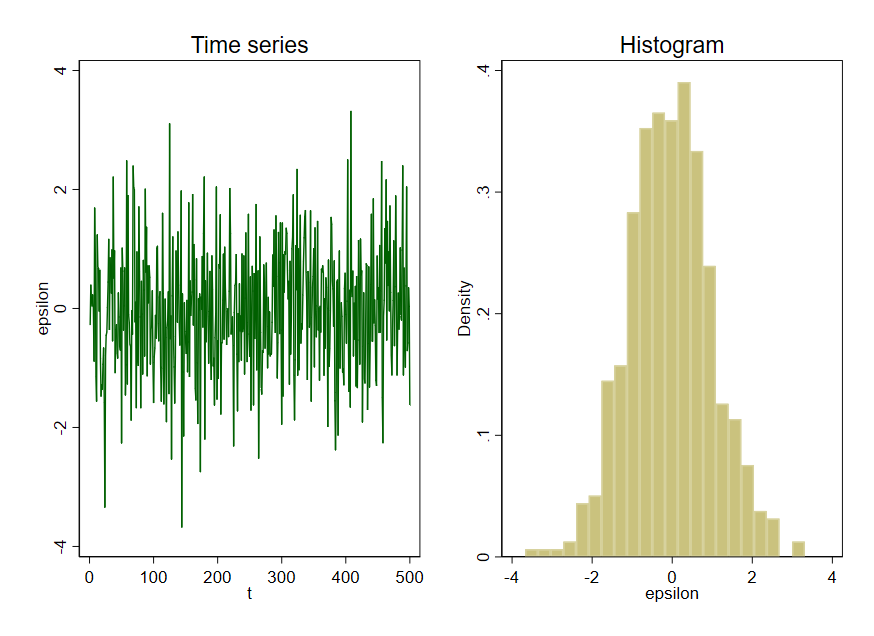
\includegraphics[width= \textwidth]{03_figures/fig22a}
  \label{fig:gaussian}
  \vspace{-2cm}
\end{figure}
\textbf{\textit{\begin{itemize}
  \item[b)] Generate AR(1) processes with three different autoregressive coefficients $\bm{\phi=\{0.5,0.8,0.95\}}$
\end{itemize}}}\noindent
Keeping the sample size at 500 and including a burn-in period of 2.000 iterations, the time series for the autoregressive models are plotted in figure \ref{fig:ar1}. The autocorrelation functions and partial autocorrelation functions are plottes in figure \ref{fig:ar1_acf}.
\\ \\
While all three processes are mean-reverting as the stationarity condition $|\phi|<1$ is fulfilled, it is clear that persistence increases as $\phi\rightarrow1$. This translates into longer lasting and more extreme cycles in figure \ref{fig:ar1} as the autoregressive element dominates the stochastic error term. Likewise, the autocorrelation functions (ACFs) show that temporal dependence is significant three periods back for $\phi=0.5$ while the autocorrelation is significant for the past 12-13 periods for $\phi=0.95$. While I have only shown 25 lags in the figures, extending it even shows that the the latter process is borderline-significantly but negatively autocorrelated with period 30-37 as well.

Figure \ref{fig:ar1_acf} shows for the ACFs as well as for the partial autocorrelation functions (PACFs) that the coefficient of correlation with the first lag is close to the actual $\phi$-values in the DGP. Except for a few outliers, the PACFs are inconsistent with AR(p) models of order $p>1$.

As the number of lags lags that are significantly autocorrelated are much higher in the ACFs as opposed to the PACFs this indicate that the processes are AR(1) and not MA(q) or ARMA(1,q) processes.
\begin{figure}[H]
  \caption{AR(1) processes with different autocorrelation coefficients}
  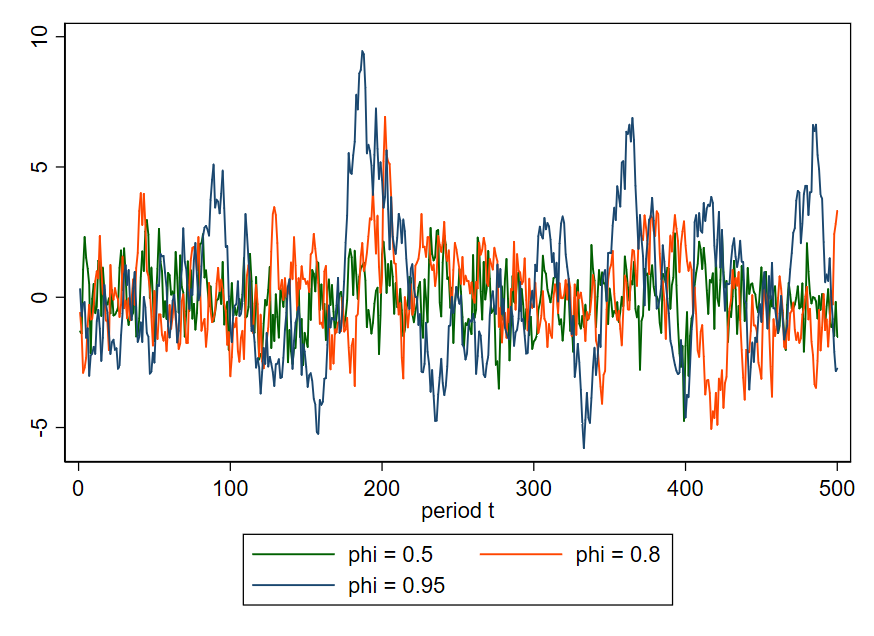
\includegraphics[width= \textwidth]{03_figures/fig22b}
  \label{fig:ar1}
  \vspace{-1cm}
\end{figure}
\begin{figure}[H]
  \caption{Autocorrelation and Partial Autocorrelation functions for AR(1) processes}
  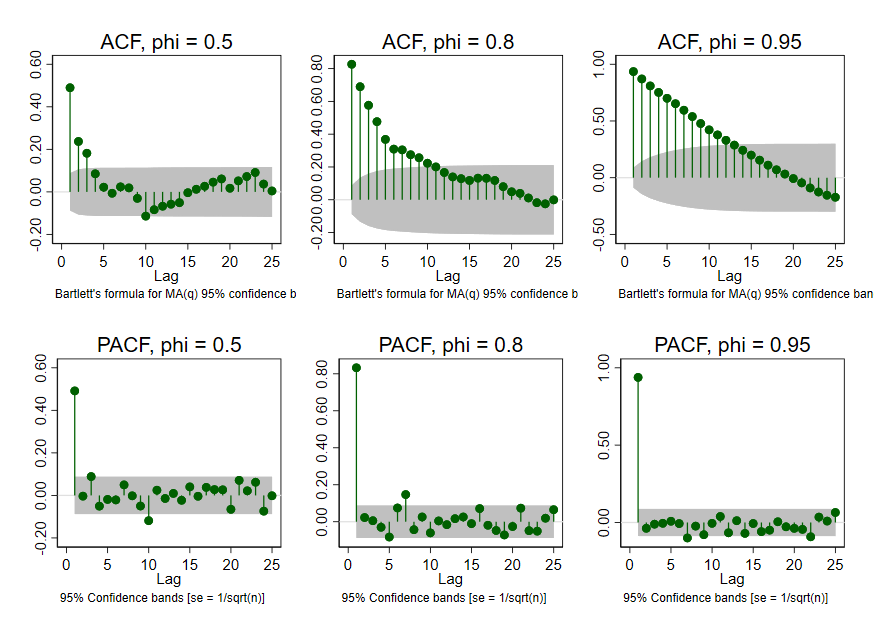
\includegraphics[width= \textwidth]{03_figures/fig22b_ac}
  \label{fig:ar1_acf}
  \vspace{-1cm}
\end{figure}
% MA(1)
\textbf{\textit{\begin{itemize}
  \item[b)] Generate MA(1) processes with three different moving average coefficients $\bm{\theta=\{0.5,0.8,0.95\}}$
\end{itemize}}}\noindent
The Moving Average processes are likewise generated with a sample size at 500m including a burn-in period of 2.000 iterations. The time series are plotted in figure \ref{fig:ma1} and the autocorrelation functions and partial autocorrelation functions are plottes in figure \ref{fig:ma1_acf} on the next page.
\\ \\
As opposed to the AR(1) processes there are as good at no signs of persistence in the time series for the MA(1) processes. Though a bit difficult to tell from comparison of figure \ref{fig:gaussian} and \ref{fig:ma1}, the summary statistics show that the standard deviation is a little higher for the MA(1) processes than for the standard normal distribution, and increase slightly with $\theta->1$.

The ACFs in figure \ref{fig:ma1_acf} confirms that there are not any persistence after the 1st lag, while the PACFs show significant lags besides the first but with alternating sign. For $\theta=0.5$ $x_t$ is linearly correlated with $x_{t-1},\ x_{t-2}$ and $x_{t-3}$ and arguably with $x_{t-3}$ (border-line significant). The MA(1) process with $\theta=0.95$ on the other hand shows significant correlation with all lags 1-8.

The number of significant lags are much higher in the PACFs as opposed to the AACFs where only the first lag is significant which is consistent with an MA(q) model of order $q=1$ while inconsistent with the processes being AR(p) or ARMA(p,q) processes.
\begin{figure}[H]
  \caption{MA(1) processes with different autocorrelation coefficients}
  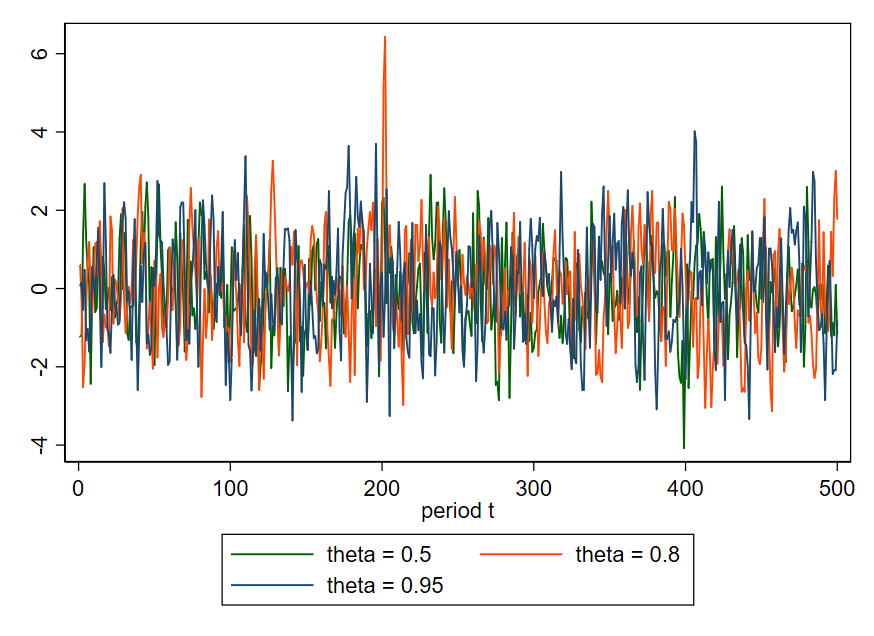
\includegraphics[width= \textwidth]{03_figures/fig22c}
  \label{fig:ma1}
  \vspace{-0.1cm}
\end{figure}
\begin{figure}[H]
  \vspace{-1cm}
  \caption{Autocorrelation and Partial Autocorrelation functions for MA(1) processes}
  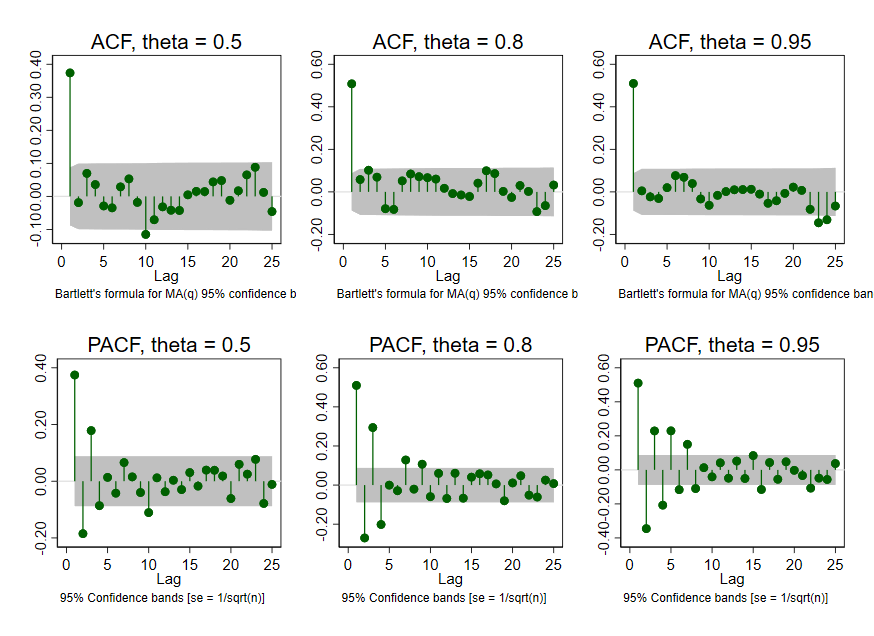
\includegraphics[width= \textwidth]{03_figures/fig22c_ac}
  \label{fig:ma1_acf}
  \vspace{-1cm}
\end{figure}
